\documentclass[sigplan]{acmart}\settopmatter{printfolios=true,printccs=false,printacmref=false}

\acmConference[NCSU, FALL 2018]{CSC512 - Compiler Construction}{October 18, 2018}{Raleigh, NC, USA}
\acmYear{2018}
\acmISBN{} % \acmISBN{978-x-xxxx-xxxx-x/YY/MM}
\acmDOI{} % \acmDOI{10.1145/nnnnnnn.nnnnnnn}
\startPage{1}
%\renewcommand{\baselinestretch}{1.00} 


\setcopyright{none}

\usepackage{booktabs}   %% For formal tables:
                        %% http://ctan.org/pkg/booktabs
\usepackage{subcaption} %% For complex figures with subfigures/subcaptions
                        %% http://ctan.org/pkg/subcaption

\usepackage{listings}
\begin{document}

%% Title information
\title[Final Course Project Report]{Final Course Project Report}         
\subtitle{SPARK API Converter}                    


\author{Md Rayhanur Rahman}
\authornote{unity id: 200255928}          %% \authornote is optional;
                                        %% can be repeated if necessary
\orcid{nnnn-nnnn-nnnn-nnnn}             %% \orcid is optional
\affiliation{
  \position{Ph.D. Student}
  \department{Dept. of CSC}              %% \department is recommended
  \institution{NC State University}            %% \institution is required
  \city{Raleigh}
  \state{NC}
  \country{USA}                   %% \country is recommended
}
\email{mrahman@ncsu.edu}          %% \email is recommended

\author{Mohammad Maruful Haque}
\authornote{unity id: 200262103}          %% \authornote is optional;
%% can be repeated if necessary
\orcid{nnnn-nnnn-nnnn-nnnn}             %% \orcid is optional
\affiliation{
	\position{Ph.D. Student}
	\department{Dept. of CSC}              %% \department is recommended
	\institution{NC State University}            %% \institution is required
	\city{Raleigh}
	\state{NC}
	\country{USA}                    %% \country is recommended
}
\email{mhaque3@ncsu.edu}          %% \email is recommended


\begin{abstract}
This document contains the final report of the SCALA API Converter project which is a course project requirements of CSC512 - Compiler Construction course. The documents highlights the problem definition, motivation, background, related work, methodology, workload distribution, results, limitations and future work direction.
\end{abstract}

\maketitle


\section{The Problem}
In this project, we need to build a source code converter which can transform these following things along with some additional tasks. 
\begin{enumerate}
	\item \textbf{RQ1:} Getting introduced with Apache Spark, setting it up in a docker container and writing some piece of code in Spark RDD, Dataset and Dataframe API. In the project requirement document, it is referred as Part 0
	\item \textbf{RQ2:} Transforming Spark RDD API to Spark Dataset API. In the project requirement document, it is referred as Part 1
	\item \textbf{RQ3:} Transforming Spark RDD API to Spark Dataframe API. In the project requirement document, it is referred as Part 2
	\item \textbf{RQ4:} Implementing some Spark SQL API calls to Scala functions and providing thoughts on how to implement a generic transformer that can transform Scala functions to corresponding SQL code.  In the project requirement document, it is referred as Part 3
\end{enumerate}

\section{Background and Motivation}
%TODO 
...Write as much detail as POSSIBLE of Spark and its corresponding APIs.
%TODO
... for the motivation part, write why this type of projects are useful

Spark is very popular these days for distributed computing tasks such as data analysis, graph modeling and machine learning etc. There are three APIs in Spark at present named RDD, Dataset and Dataframe. The three different APIs provide different expressive power to achieve the same thing although the performance gain can be different. Moreover, Spark introduced these three APIs in different times so that there are many existing implementations of Spark based systems that needs to be rewritten to gain better performance. So, an API transformer can be handy to migrate Spark APIs to achieve better performance. Moreover, by doing this, a great understanding will be built on compiler techniques such as scanning and parsing, handling CFG grammar and intermediate representation.  

\subsection{Motivation}
The problem we are about to work upon largely falls into the domain of source to source compiler or transcompiler. It is a type of compiler where the source code of a program written in one programming language is taken as input and the equivalent source code in another programming language is produced as an output. It is different from traditional compiler in a sense that source-to-source compilers converts one programming language to another where both of those belongs to the same abstraction level whereas a conventional compiler turns a high level language to a low level one. These types of compiler is also useful in case of 
\begin{itemize}
    \item transforming legacy code base to a modern counterpart such as structured to OOP design \cite{zou2001framework}
    \item transforming to newer set of APIs or maintaining issues with backward compatibility
    \item transforming code in more modular version
    \item porting a code to different platforms
    \item reducing technical debt of code base by applying automatic refactoring
    \item developing new language on top of existing and established language such as \textit{typescript} running on top of \textit{javascript}
\end{itemize}

In our context, it is already known that, in terms of performance, $dataframe > dataset > RDD$. Hence, a legacy distributed computing focused application written in \textit{Spark RDD} API can be transformed to \textit{Dataset} or \textit{Dataframe} API to extract the best performance from the computing devices. If we can build an automatic transcompiler that can perform aforementioned duty, then it could save a considerable amount of human effort and brings out better performance at the same time. 

\section{Related Work}
%TODO
...find some papers


\section{Methodology}
In this section, the step by step process for each of the task is described below:

\subsection{RQ1}
%TODO
...write description for RQ1. Describe the test setup, write something about docker environment... step by step process... give examples of two of each three APIs..

\subsection{RQ2}
\subsubsection{Execution Environment}
We implemented a python program that can handle the requirements stated in RQ2. Our machine was a typical laptop computer. Here is the description of the execution environment.

\begin{table}[]
\begin{tabular}{|l|l|lll}
\cline{1-2}
Operating System & Arch Linux           &  &  &  \\ \cline{1-2}
Kernel Version   & 4.19                 &  &  &  \\ \cline{1-2}
Python Version   & 3.7                  &  &  &  \\ \cline{1-2}
Processor        & Core i7 8550U 1.8GHz &  &  &  \\ \cline{1-2}
Memory           & 16 GB 2400 MHz       &  &  &  \\ \cline{1-2}
DIsk             & 240GB SSD            &  &  &  \\ \cline{1-2}
\end{tabular}
\caption{Execution Environment for RQ2}
\label{tab:env}
\end{table}

\subsubsection{Libraries}
We used raw pythond codes to do the task. No additional library modules were used to achieve the goal for this task.

\subsubsection{The Goal}
For this following input:
\begin{lstlisting}
sc.range(1,10000000)
.map(i=>(i%11, 1))
.reduceByKey((a:Int, b:Int) => a+b)
.collect()
\end{lstlisting}

We need to produce the following output:
\begin{lstlisting}
spark.range(1,10000000)
.map(i=>(i%11, 1))
.groupByKey(_._1)
.agg(reduceByKeyAggregator((a:Int, b:Int) 
=> a+b))
.collect()
\end{lstlisting}

\subsubsection{Algorithm}
Here is the step by step process on how we achieved the requirements of RQ2.


\begin{figure}[h]
	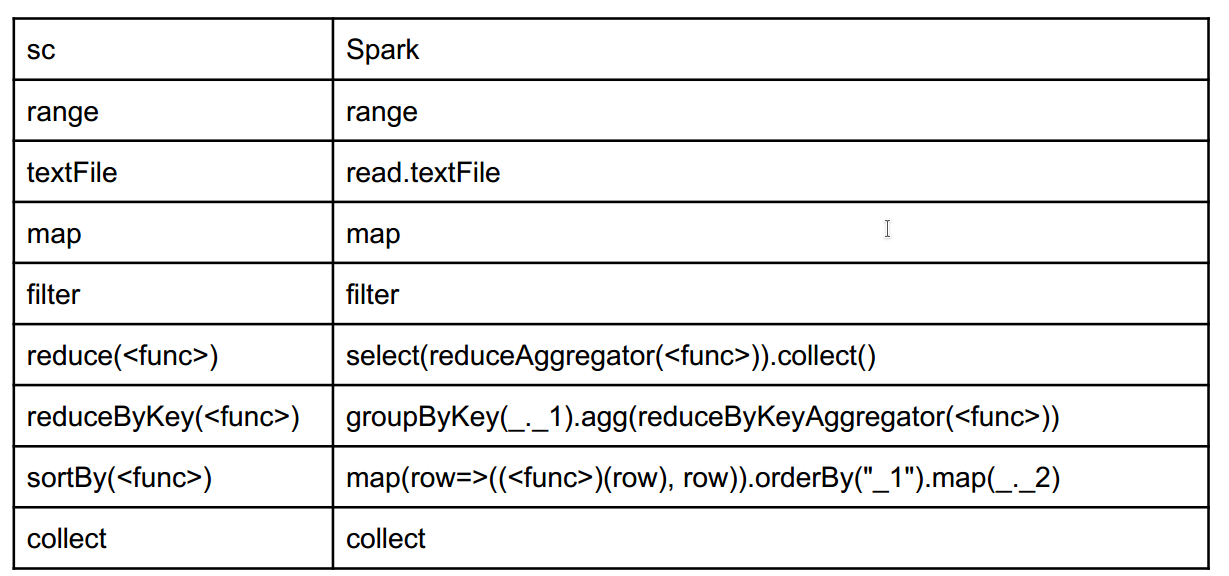
\includegraphics[width=6cm,height=4cm,keepaspectratio]{fig/t1.png}
	\caption{Transformation Rules}
	\label{fig:token}
\end{figure}

\begin{lstlisting}[caption=token definition, label=list:token]
<letter> --> a | b | ... | y | z 
| A | B | ... | Z | 
<digit> --> 0 | 1 | ... | 9
<number> --> <digit>+
<identifier> --> <letter> (<letter> 
| <digit>)*
<string> --> any string between (and 
including) the closest pair of double 
quotation marks.
<char> --> a character between (and 
including) a pair of single quotation 
marks.
<symbol> --> any non-space character 
that is not a part of other tokens
\end{lstlisting}

\begin{enumerate}
    \item First we took the whole input as a simple python string object. 
    \item We filtered all the new line, carriage returns and tabs from that string
    \item We wrote regular expression checker using python's default \textit{re} module for the following tokens highlighted in list \ref{list:token}
    \item After that, we read the whole string one character at a time and tokenized the whole string
    \item we replaced the tokens according to the transformation rules mentioned above
    \item just replacing the tokens does not actually do the whole job. We needed to match the opening brackets and closing brackets associated with each of the tokens and then we replaced the tokens and appended corresponding tokens after the right parenthesis according to the transformation rules
\end{enumerate}

\subsubsection{Sample Test Cases}
%TODO
... put some test cases here

\subsubsection{Discussions}
Here is some of the observation we came through while implementing the RQ2.
\begin{itemize}
    \item Our transformed would not work if there will be any identifier having names that is present in the transformation table. For example, this following statement will produce an error.
    \begin{lstlisting}
        map(x => sc)
    \end{lstlisting}
    Because \textit{sc} is already in the transformation table.
    \item This phenomenon happens because the transformed would not know if the \textit{sc} is an identifier or an object. This aforementioned problem could have been solved if we could have constructed the whole grammar for the Spark RDD API. But developing a full fledged grammar was an infeasible task, hence we did not implemented it. If the grammar was there, then it was fully possible to first parsing the tokens, building an abstract syntax tree and replace the nodes with corresponding nodes according to the transformation rules. 
\end{itemize}

\subsection{RQ3}
\subsubsection{Execution Environment}
The environment details are as same as Table \ref{tab:env}.

\subsubsection{Libraries}
Initially we planned to build the whole transformer, (i.e. scanner, parser, tree) from scratch. Later, we found out that there are some existing excellent framework for doing these types of tasks with \textit{ANTLR, YACC, JavaCC, Scala Parser Combinators} etc. However, finally we choose a framework named \textit{Lark} which is written in pure Python to generate scanners and parsers for our goal. Lark can:
\begin{itemize}
    \item Parse all context-free grammars, and handle all ambiguity
    \item Build a parse-tree automatically, no construction code required
    \item Outperform all other Python libraries when using LALR(1) (Yes, including PLY)
    Run on every Python interpreter (it's pure-python) Generate a stand-alone parser (for LALR(1) grammars)
\end{itemize}

We didn't choose the De Facto \textit{ANTLR} as it is heavy and initial learning curving is a bit steep despite being a powerful framework for these type of tasks. 

\subsubsection{The Goal}
For the following input, 
\begin{lstlisting}
sc.range(10,100)
.map(i=>{val j=i%3;
(i, if(j==0)i*10 else i*2)})
.map(r=>r._1+r._2)
.collect()
\end{lstlisting}
We have to produce the following output,
\begin{lstlisting}
spark.range(10,100).selectExpr("id as _1")
.selectExpr("_1 as _1", 
"if(_1%3==0,_1*10,_1*2) as _2")
.selectExpr("_1+_2 as _1")
.collect()
\end{lstlisting}

\subsubsection{Algorithm}
The step by step process to achieve the goal stated in RQ3 is mentioned below.

\begin{lstlisting}[caption=UDF Grammar, label=list:g1]
<Program> ::= sc.range(<number>,<number>)
<MapOps>.collect()
<MapOps> ::= epsilon | <MapOps>.map(<UDF>)
<UDF> ::= <identifier> => <Expression>
<Expression> ::= {<ComplexExpr>} 
    | <SimpleExpr>
<SimpleExpr> ::= <PureExpr> 
    | (<TupleExpr>)
<TupleExpr> ::= <PureExpr>, <PureExpr> 
| <TupleExpr>, <PureExpr>
<ComplexExpr> ::= <SimpleExpr> 
    | <AssignExprs>;<SimpleExpr>
<AssignExprs> ::= <AssignExpr> 
    | <AssignExprs>;<AssignExpr>
<AssignExpr> ::= val <identifier> = 
<PureExpr>
<PureExpr> ::= <identifier> 
    |<identifier>.<identifier> 
    |(<PureExpr>) 
    |<PureExpr> <Op> <PureExpr> 
    |if ( <CompExpr>) <PureExpr> else 
    <PureExpr>
    <CompExpr> ::= <PureExpr> <Comp> 
    <PureExpr>
    <Op> ::= + | - | * | %
<Comp> ::= == | < | > | != | >= | <=
\end{lstlisting}

\begin{lstlisting}[caption=lark grammar, label=list:g2]
// rdd grammar
start : SC actions*
    actions : DOT RANGE LP rangeparams* RP
            | DOT TEXTFILE LP URI RP
            | DOT MAP LP func RP
            | DOT FILTER LP func RP
            | DOT REDUCE LP func RP 
            | DOT REDUCEBYKEY LP func RP
            | DOT SORTBY LP func RP
            | DOT COLLECT LP RP

    rangeparams : NUMBER (COMMA NUMBER)?


    func : ID ARROW expression
    expression : simpleexpression
               | LB complexexpression RB
    simpleexpression : pureexpression
                     | LP tupleexpression RP
    tupleexpression : pureexpression COMMA 
                    pureexpression 
                    | tupleexpression COMMA 
                    pureexpression
    complexexpression : simpleexpression
                      | assignmentexpressions 
                      SEMICOLON 
                      simpleexpression
    assignmentexpressions : 
    assignmentexpression 
    | assignmentexpressions SEMICOLON 
    assignmentexpression
    assignmentexpression : 
    VAL ID EQUAL pureexpression
    pureexpression : NUMBER
                   | ID
                   | ID DOT ID
                   | LP pureexpression RP
                   | pureexpression OP 
                   pureexpression
                   | IF LP 
                   comparisonexpression 
                   RP pureexpression 
                   ELSE pureexpression
    comparisonexpression : pureexpression 
                    COMP pureexpression

    SC : "sc"
    VAL : "val"
    IF : "if"
    ELSE : "else"
    EQUAL : "="
    DOT : /[.]/
    OP : /[ ]*["+"\-*""%"][ ]*/
    COMP : ( /[ ]*[=][=][ ]*/ 
    | /[ ]*[>][ ]*/ | /[ ]*[<][ ]*/ 
    | /[ ]*[!][=][ ]*/ 
    | /[ ]*[>][=][ ]*/ 
    | /[ ]*[<][=][ ]*/ )
    COMMA : /[,]/
    SEMICOLON : /[;]/
    ARROW : /[ ]*[=][>][ ]*/
    LB : /[ ]*[{][ ]*/
    RB : /[ ]*[}][ ]*/
    LP : /[ ]*["("][ ]*/
    RP : /[ ]*[")"][ ]*/
    RANGE : "range"
    TEXTFILE : "textFile"
    MAP : "map"
    FILTER : "filter"
    REDUCE : "reduce"
    REDUCEBYKEY : "reduceByKey"
    SORTBY : "sortBy"
    COLLECT : "collect"

    URI : ( /["\""]/ | /["'"]/ ) 
    /[\\\a-zA-Z.:\/]*/ 
    ( /["\""]/ | /["'"]/ )
    //FUNC : "<func>"

    %import common.CNAME -> ID
    %import common.SIGNED_NUMBER 
    -> NUMBER
    %import common.WS
    %ignore WS
\end{lstlisting}

\begin{figure}[h]
	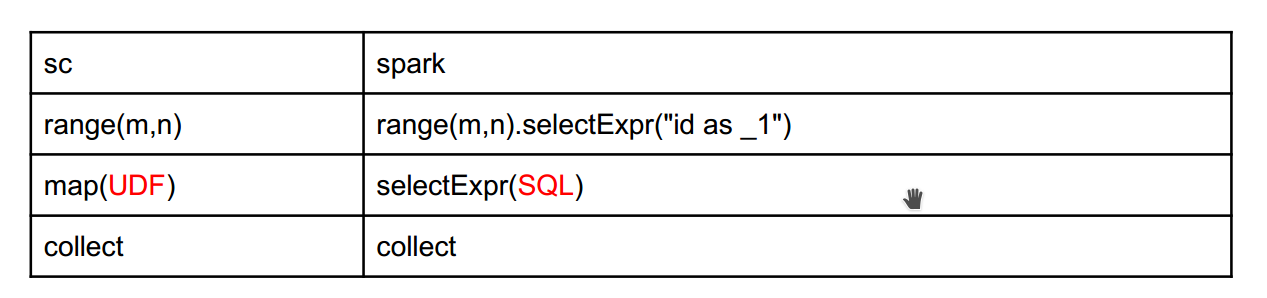
\includegraphics[width=6cm,height=4cm,keepaspectratio]{fig/t2.png}
	\caption{Transformation Rules}
	\label{fig:t2}
\end{figure}

\begin{figure}[h]
	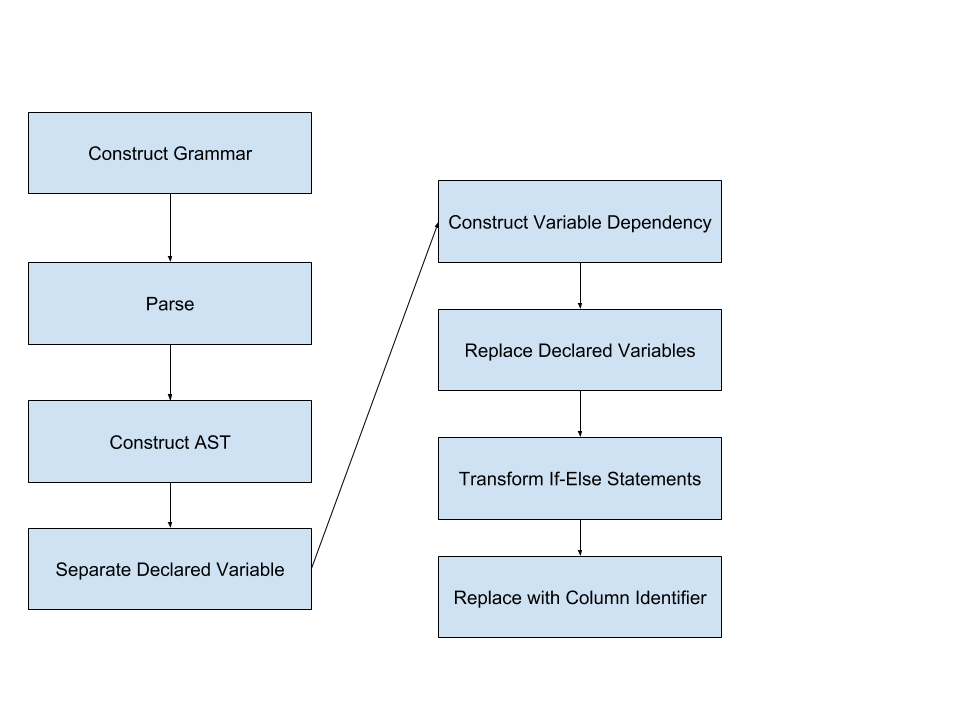
\includegraphics[width=6cm,height=4cm,keepaspectratio]{fig/d.png}
	\caption{Flowchart of RQ3}
	\label{fig:d}
\end{figure}

\begin{enumerate}
    \item First, we need to have a grammar upon which the parser and abstract syntax tree will be built upon. The grammar has been given in the list \ref{list:g1}
    \item As we used \textit{lark-parser} for the task of parsing and generating abstract syntax tree, we needed to transform the grammar to feed into the lark-parser convention. That grammar is given in list \ref{list:g2}
    \item we developed an abstract syntax tree on top of the \textit{lark-parser}. 
    \item we extracted the tokens which were needed to be replaced according to the transformation rules given in figure \ref{fig:t2}
    \item the most challenging part is obviously transforming the UDF to SQL. There are actually two source of difficulties in transforming UDF to SQL. First one is to figure out the dependencies of the variables of \textit{AssignExprs}. The second one is to convert the \textit{if-else} portion of the UDF to corresponding SQL syntax. 
    \item For the first challenge, we extracted the UDF portion from the input first. Then we separated the variable declaration part from the rest of the expression. Then we determined the dependency of the variables and replaced all the variables with appropriate mathematical expression. At the end, all the declared variables were replaced. 
    \item For the second challenge, we parsed the \textit{if-else} and nested \textit{if-else} statements using a \textit{stack} based data structures. Then we replaced all the variables of conditions with the root variable that came from the input of the lambda expression. \item Finally, we replaced the input variables with Spark SQL column identifier such as \textit{\_1, \_2} etc.
\end{enumerate}

The whole step by step process is also represented as flowchart in figure \ref{fig:d}.

\subsubsection{Sample Test Cases}
%TODO
...provide some sample test cases

\subsubsection{Discussion}
Here is some observation we came through while implementing RQ3.

\begin{itemize}
    \item Our implementation only works for the simple UDF functions as provided in the grammar described in the project requirements
    \item Our implementation contains parenthesis to preserve the meaning of mathematical formulas. In some cases, those brackets were redundant though.
    \item Handling the nested \textit{if-else} was particularly challenging. 
    \item We assume that, there might be a more elegant solution to achieve the goal of RQ3. For example, the whole thing could have done recursively using abstract syntax tree and intermediate code representation. For example, a directed acyclic graph could have been drawn to identify the data flow and variable dependencies. 
    \item Moreover, the nested \textit{if-else} statements could have automatically constructed with the abstract syntax tree. After that, a recursive transformer could have converted those expression to corresponding SQL statements. 
\end{itemize}

\subsection{RQ4}
%TODO
... same as RQ1

\subsubsection{How a Generic Scala to SQL Transformer can be Built}
Although, in this course project, we have implemented a simple transformer that can basically transform simple UDF in lambda queries to Spark SQl syntax. But, that can be generalized to whole bunch of full fledged scala lambda queries to SQL. In order to do that, we can build an expression tree which will contain each lambda expressions \textit{left}, \textit{operator}, \textit{right} and the \textit{node type} information. Expressions can be of these following types: 
\begin{itemize}
    \item \textbf{unary:} An operation with a single operand such as negation
    \item \textbf{binary: }An operation with two operands such as addition or \&\& or ||.
    \item \textbf{parameter: }An input to a lambda function
    \item \textbf{member: }Accessing a property, field, or method of an object or a variable. 
    \item \textbf{constant: }A node that is a constant value
\end{itemize}

After constructing the tree, we can recursively traverse each nodes and generate the equivalent SQL queries for each nodes. For example, if a node contains \textit{startsWith} method, we can generate the SQL query contain \textit{LIKE} operator. However, it might be the case that not all Scala operations are automatically transformable to the corresponding SQL queries, i.e., custom functions. 

\section{How to setup Testing Environment}
The transformer program is standalone and self packaged. Hence, there is no need for configuration or settings file. It is designed in such a way so that the tester can test it by just running the scripts and providing appropriate input files. Custom test cases can be written as well to test some sample inputs and outputs. The code samples as input and produced output code samples must preserve the same meaning and produce the same result according to the transformation table. That is the key testing criteria. Our test programs for Part 0 and Part 3 are written in Scala. For the part 1 and part 2, the test programs are written in Python. Here are the requirements to run the test programs.

\begin{itemize}
    \item Linux or Mac OSX
    \item Docker container where Apache Spark has been setup
    \item Python3
    \item \textit{lark-parser} python package 
\end{itemize}

\section{Workload Distribution}
After completing the whole task, here is the workload distribution for our team.
\begin{itemize}
    \item Part 0: Done by Maruful
    \item Part 1: Done by Rayhanur
    \item Part 2: Done by Rayhanur and Maruful
    \item Part 3: Done by Maruful and Rayhanur
\end{itemize}










%% Bibliography
\bibliography{bibfile}
\bibliographystyle{ACM-Reference-Format}
%
%
%%% Appendix
%\appendix
%\section{Appendix}


\end{document}
